% =============================================================================
% Autore originale: Fabio Tempera
% Licenza: MIT (vedere LICENSE nel medesimo direttorio)
%
% DOCUMENTO
%   Una pagina di presentazione della rete TESS-4C, da distribuire allo stand
%   CieloBuio OdV alla Fiera Astroshow di Cesena (7 e 8 novembre 2026).
%   Il codice QR, da generare a cura del gruppo che cura il sito, rimanda al
%   testo di presentazione pubblicato su CieloBuio OdV.
%
% COMPILAZIONE
%   pdflatex fiera-cesena.tex  (due passate per i riferimenti alla Figura)
%   Classe report, pacchetti in packages.sty. Non usare Markdown.
% =============================================================================

\documentclass[11pt,a4paper]{report}

\usepackage{packages}

\definecolor{nightblue}{RGB}{22,38,58}
\definecolor{steel}{RGB}{80,100,120}

\geometry{a4paper, top=1.6cm, bottom=1.4cm, left=2.2cm, right=2.2cm}

\pagestyle{empty}
\setlength{\parskip}{0.35em}

\hypersetup{
  colorlinks=true,
  urlcolor=nightblue,
  pdftitle={Rete TESS-4C. Presentazione per la Fiera Astroshow di Cesena},
  pdfauthor={Fabio Tempera}
}

\newcommand{\titolino}[1]{%
  \par\vspace{0.5em}
  \noindent{\normalsize\bfseries\color{nightblue} #1}\par
  \vspace{0.05em}
}

\begin{document}

\begin{center}

{\LARGE\bfseries\color{nightblue} Una stazione per il cielo notturno\par}

\vspace{0.2cm}

{\large Misurare il buio, insieme\par}

\vspace{0.2cm}

{\small CieloBuio OdV, progetto rete TESS-4C\par}

\vspace{0.2cm}

{\small Stand CieloBuio OdV, Astroshow, Fiera dell'Astronomia di Cesena, 7 e 8 novembre 2026\par}

\end{center}

\titolino{Il problema}

L'inquinamento luminoso riduce la visibilità del cielo stellato e incide su ecosistemi e consumi energetici. Per valutare le norme regionali e gli effetti delle sostituzioni dell'illuminazione servono misure a terra, continue e confrontabili nel tempo.

\titolino{Lo strumento}

Il TESS-4C è un fotometro a 4 bande, da installare all'esterno con vista libera sullo zenit. Trasmette i dati via WiFi all'archivio aperto della rete STARS4ALL e a un cruscotto gestito da CieloBuio OdV. Il costo indicativo è di 550-650 EUR, IVA e spedizione comprese.

\titolino{La proposta}

Il progetto si rivolge a gruppi astrofili, scuole, centri culturali e amministrazioni comunali. Vi interesserebbe acquistare uno strumento, che resterebbe nella disponibilità del vostro gruppo o ente, e far parte della rete? Lasciate la vostra email allo stand oppure scrivete a \url{fabiot2801@gmail.com} o inviate un messaggio WhatsApp al numero 329 883 5142. Seguirà un incontro online di circa 30 minuti, dedicato ai dettagli del progetto. Una risposta di interesse non comporta alcun impegno.

\begin{figure}[ht!]
\centering
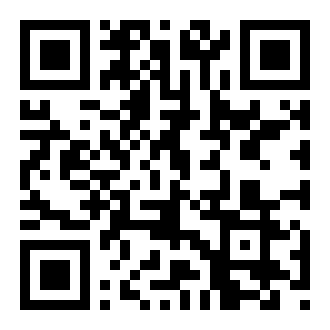
\includegraphics[width=3.4cm]{figures/qr-esempio.png}
\caption{Codice QR di rimando al testo di presentazione sul sito di CieloBuio OdV.}
\label{fig:qr}
\end{figure}

\noindent Fabio Tempera, CieloBuio OdV

\end{document}
